\chapter{Evaluation}
\label{chap:eva}
\section{Setup}
The CLONALG algorithm will be applied to a set of 17 different TSP problems from the TSP library TSPLIB95 \footcite[https://www.iwr.uni-heidelberg.de/groups/comopt/software/TSPLIB95/]{tsplib}. The implementation follows the specification in \cite{DEC02} and is provided by the OAT \footcite[http://optalgtoolkit.sourceforge.net/]{oat}. The greedy search algorithm will be applied to the same set of problems. This algorithm is provided by the author of the OAT and uses a nearest neighbour technique with mutation and it is quite effective in solving the provided TSP.\\\\ 
The stopping criteria for the algorithm will be no improvements after a set amount of evaluations. No improvement means that the algorithm has not found a shorter route in it's actual iteration compared to the last one, this is often also called stagnation. 
The criteria for the results are:
\begin{enumerate}
	\item 	Score
	\item 	Time in ms
	\item 	Evaluations	
	\item  	Percentage of optimal score
\end{enumerate}
Percentage of optimal score is the difference to the best possible route of the TSP. The score is measured as the summarized Euclidean distance of the presented best tour. The algorithm will be run multiple times on one TSP therefore the arithmetic mean of each criteria will be the end result. To compare the results the mean average error (MAE) of the average score will be used. The MAE is composed from the difference between the score of both algorithms divided through the score of the main compared algorithm, if we want to compare the performance of algorithm A1 to A2 the MAE is calculated as $(A2-A1)/A1$. Positive MAE means better performance for A1. The significance of the difference is visible at the digit. The thousands digit shows no significant difference. This was tested by running the complete test run twice on the same algorithm. The single test runs only had a difference visible on the thousands digit. Differences on the hundreds and tens digit are significant. The CLONALG algorithm will be applied to the problem set multiple times with different parameters. The adaptive algorithms will be applied only once because of the dynamic parameters.
The parameters which will be altered are
\begin{enumerate}
	\item 	Population size
	\item 	Clone factor
	\item 	Selection size
	\item 	Random replacements	
\end{enumerate}
The first set of parameters will be the default parameters provided by the OAT as shown in table \ref{tuning}. The second one are the parameters that are proposed by DeCastro [DEC02] for solving TSP problems about the size of 30 nodes.
The adaptive variant of the CLONALG algorithm will use the default vaulues at the beginning and adjust the paramaters during runtime.
To measure the results, a modified version of the optimization algorithm toolkit (OAT) [2] will be used. The changes are a slightly different set of TSP Problems used in the domain and the addition of an adaptive CLONALG hybrid algorithm. The used TSP problems are listed in the appendix. The distances between the nodes in the TSP problem are measured as Euclidean distance. The implemented CLONALG algorithm is based on the specifications in \cite{DEC02}. The adaptive variant expand the concept based on \cite{Garret04}.
Both algorithms will be applied 100 times on every single TSP problem.\\\\
The hardware is a i5-3320M dual core CPU with 2,60ghz each and 8gb of RAM, run on a Windows 10 operating system with only the necessary windows background tasks. All CPU and RAM usage shown in this thesis is after other processes, not related to the algorithm, are taken into account.
\subsection{Evolution Strategy Parameter Control}
The first CLONALG variation is based on \cite{Garret04} and uses an idea from the evolution strategy \cite{evolution}. The original managed to eliminate all parameters except population size from the CLONALG algorithm. This thesis uses a variant where the selection size n is eliminated. This is comparable to Variant C1-C4 from \cite{Garret04}. It uses a strategy parameter which will adjust the selection size. The strategy parameter itself will be adjusted by a evolution strategy constant of 1.3. This constant was empirically tested and proofed to be the most effective \cite{Garret04}. The adjustment is randomized, the strategy parameter will be either multiplied or divided by the constant based on a 50\% chance. The strategy parameter itself will alter the selection size on each evaluation. The evolution strategy calls this evolution approximated by self evolution, however the difference to the original evolution strategy is, that a parameter is indirectly adjusted through another parameter \cite{Garret04}. Naturally the selection size still has to be initialized and can't be zero. \cite{Garret04} proposed to start with a small number, the test runs in this thesis start with a selection size of 1. Another difference to the orignial CLONALG is the absence of random replacements. The population will only be altered by the clones and their mutations. The changes made to the original pseudo code in chapter \ref{chap:ais} are shown in algorithm \ref{algo2}. This variant will be called CLONALG ESPC, short for Evolution Strategy Parameter Control.\\\\
\begin{algorithm}[H]
	Set strategy paramater Sp\\
	Generate initial population C of A antibodies\\
	Oc=Calculate Fitness(C)\\
	\While{stopping criteria not met}{
		S= Select the n best antibodies from C\\
		P= Generate clones of the antibodies in S\\
		Mutate(P)\\
		C= Select the n best antibodies out of P\\
		C= C + New population A-n\\
		If C has better fitness than Oc then\\
		n=Sp * 1.3 OR n= Sp/1.3\\
		else\\
		n=n\\
		end if\\
	}
	\caption{CLONALG variant with dynamic selection size}
	\label{algo2}
\end{algorithm}
\section{Results}
\subsection{CLONALG un-tuned}
The algorithms are run 100 times on every TSP. The stopping criteria are no improvements after 10000 iterations of the algorithm. This number is chosen to give the algorithm enough time without restricting it to a specific amount of seconds. The CPU usage spiked around 58\% and was average around 30\% for all algorithms. This is because the more costly operations like sorting, selection, cloning and mutation will be done in exactly the same way in all algorithms.\\
The parameters for the original CLONALG are shown in Table \ref{tuning}.\\
The parameter C is the initial population, n is the selection size for cloning, B is the cloning factor (how many clones of the chosen n will be done) and d are the random replacements to keep the new population partially randomized. \cite{DEC02} proposed some tuning to the default parameters for more efficiency in solving TSP. The replacement value d should always be between 5-20\% of the population. Higher ratios tend to randomize too much while lower ratios can still produce good results but less reliable and efficient as shown in \cite{DEC02}.\\\\
\begin{table}[H]
	\begin{tabular}{|c|c|c|c|c|}
		\hline
		& C   & n   & B   & d  \\ \hline
		Default & 50  & 50  & 0.1 & 5  \\ \hline
		Tuned   & 300 & 150 & 2.0 & 60 \\ \hline
	\end{tabular}
	\caption{Tuning parameters}
	\label{tuning}
\end{table} 
When comparing the results it is clearly seen that the CLONALG algorithm is worse on average than the greedy search algorithm as shown in table \ref{tab:clonalg_untuned}. However the CLONALG was able to find the best solution to the TSP ulysses22 with a MAE of 0.117 while the greedy search algorithm could not as shown in figure \ref{CLONALG_Avg}. The overall time for solving all problems was also shorter for the CLONALG. The number of evaluations is mostly smaller for the CLONALG which shows that stagnation started earlier in this algorithm. The average MAE for all TSP compared to the greedy algorithm is -0.524. The average MAE for all TSP calculated on the best score is in the same range with -0.546. The mean average error of -0.009 is not significant for the TSP berlin52 which highlights that CLONALG performs equal or better on small TSP under 50 nodes but is less efficient at more difficult TSP than the greedy algorithm.
\begin{figure}[H]
	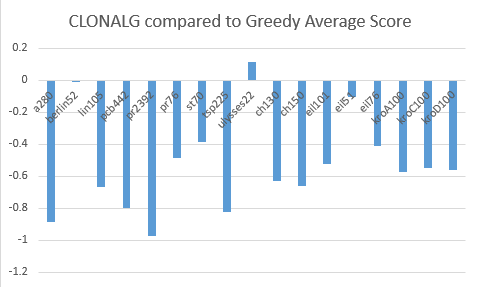
\includegraphics[]{Images/CLONALG_Fig_Avg.png}
	\label{CLONALG_Avg}
	\caption{MAE on Average Score for CLONALG compared to Greedy}
\end{figure}
\begin{table}[H]
	\begin{tabular}{|l|l|l|p{2cm}|p{2.5cm}|p{2cm}|}
		\hline
	TSP	& Avgerage Score & Best Score & Best Percentage & MAE compared to Greedy & Average Evaluations \\ \hline
		a280      & 26483.99       & 25581      & 891.8960838     & -0.885322038           & 38462.71            \\ \hline
		berlin52  & 11077.22       & 9369       & 24.22434368     & -0.009083507           & 132557.69           \\ \hline
		lin105    & 69431.08       & 62981      & 338.0068155     & -0.666910122           & 59348.99            \\ \hline
		pcb442    & 649513.41      & 631174     & 1143.006814     & -0.795694149           & 38322.66            \\ \hline
		pr2392    & 14231642.92    & 14122859   & 3635.889819     & -0.971810641           & 32506.49            \\ \hline
		pr76      & 299815.73      & 267781     & 147.5808763     & -0.486638576           & 73496.26            \\ \hline
		st70      & 1765.09        & 1510       & 123.7037037     & -0.382569727           & 82887.36            \\ \hline
		tsp225    & 31309.96       & 29905      & 663.6618999     & -0.822318521           & 41252.29            \\ \hline
		ulysses22 & 7273.04        & 6901       & 0               & 0.117078966            & 27588.51            \\ \hline
		ch130     & 31453          & 29391      & 381.0310966     & -0.630750644           & 46159.77            \\ \hline
		ch150     & 37883.24       & 36015      & 451.7003676     & -0.660824945           & 47285.45            \\ \hline
		eil101    & 2126.54        & 1954       & 210.6518283     & -0.525482709           & 56058.04            \\ \hline
		eil51     & 654.65         & 552        & 29.57746479     & -0.103093256           & 115597.85           \\ \hline
		eil76     & 1377.39        & 1194       & 121.9330855     & -0.407509856           & 67914.53            \\ \hline
		kroA100   & 96214.68       & 86675      & 307.2690537     & -0.572862998           & 60339.55            \\ \hline
		kroC100   & 94471.33       & 85368      & 311.4318762     & -0.550283351           & 60015.33            \\ \hline
		kroD100   & 93282          & 84305      & 295.9096459     & -0.557829485           & 57958.20            \\ \hline
	\end{tabular}
	\caption{CLONALG untuned performance}
	\label{tab:clonalg_untuned}
\end{table}
\subsection{CLONALG tuned}
Comparing the tuned algorithm to the original one shows, that the tuned parameter are not suited for this TSP setup. The tuned CLONALG has a worse average score in solving all 17 TSP compared to the untuned CLONALG. The unexpected outcome is, that the tuned algorithm performs better if the TSP is larger. The MAE on pr2392, which is the largest TSP in the setup, is only -0.014 but the MAE of ulysses22, the smallest TSP, is -0.305. The algorithm could not find the best solution for ulysses22. The average MAE for all TSP was -0.253 compared to the untuned algorithm. This is especially unexpected because the parameters where tuned by [DEC02] for a 30 node TSP. In their tests, the tuned algorithm behaved better on this specific TSP than the un-tuned one. This shows that the chosen parameters do not work well when the stopping criteria are 10000 evaluations without improvement.
\begin{table}[H]
	\begin{tabular}{|l|l|l|l|p{2.5cm}|p{2cm}|}
		\hline
		TSP       & Avgerage Score & Best Score & Best Percentage    & MAE compared to CLONALG & Average Evaluations  \\ \hline
		a280      & 29313.63    & 27910     & 982.202404  & -0.09652984                                                     & 12173.27 \\ \hline
		berlin52  & 22284.75    & 20861     & 176.5977194 & -0.502923748                                                    & 13140.05 \\ \hline
		lin105    & 95696.8     & 89181     & 520.2169831 & -0.274468112                                                    & 12437.46 \\ \hline
		pcb442    & 695194.14   & 680524    & 1240.194572 & -0.065709314                                                    & 12179.71 \\ \hline
		pr2392    & 14434730.31 & 14288477  & 3679.700396 & -0.014069358                                                    & 11541.92 \\ \hline
		pr76      & 445633.5    & 418899    & 287.2992539 & -0.327214561                                                    & 12718.28 \\ \hline
		st70      & 2826.17     & 2672      & 295.8518519 & -0.375448045                                                    & 12650.36 \\ \hline
		tsp225    & 35353.65    & 32603     & 732.5587334 & -0.114378289                                                    & 12485.88 \\ \hline
		ulysses22 & 10459.55    & 9389      & 36.05274598 & -0.304650774                                                    & 13776.71 \\ \hline
		ch130     & 38766.46    & 36521     & 497.7250409 & -0.188654316                                                    & 13543.46 \\ \hline
		ch150     & 45610.23    & 43708     & 569.5465686 & -0.169413529                                                    & 12907.27 \\ \hline
		eil101    & 2773.71     & 2685      & 326.8680445 & -0.233322878                                                    & 13245.55 \\ \hline
		eil51     & 1240.14     & 1170      & 174.6478873 & -0.472116051                                                    & 13879.30 \\ \hline
		eil76     & 1993        & 1806      & 235.6877323 & -0.308886101                                                    & 13296.35 \\ \hline
		kroA100   & 134148.49   & 125461    & 489.5169627 & -0.282774782                                                    & 13492.89 \\ \hline
		kroC100   & 132863.13   & 126691    & 510.5884621 & -0.288957516                                                    & 13778.59 \\ \hline
		kroD100   & 129082.57   & 124611    & 485.1930121 & -0.277346275                                                    & 14173.76 \\ \hline
	\end{tabular}
	\caption{CLONALG tuned performance}
	\label{tab:clonalg_tuned}
\end{table}
\subsection{CLONALG ESPC}
The variant with an adaptive selection size shows only a insignificant worse performance with an average MAE for all TSP of -0.009. The interesting behaviour is seen in the average MAE for all TSP calculated on the best score with 0.039. This value shows that the adaptive CLONALG is better in finding the shorter route but will also produce some worse ones in the long run. The MAE on the best score was significant better on eil101, kroA100 and kroD100 which are bigger TSP. This results highlights that a adaptive selection size altered with the evolution strategy and combined with no random replacements can be beneficial for finding the shorter route. On average the CLONALG ESPC needed less evaluations to terminate, the stagnation started earlier in this variant. The overall runtime was nearly identical for the original CLONALG and the ESPC with close to 19 minutes for the complete run. Comparing the ESPC to the greedy algorithm still shows a worse performance on average and in most cases on best score for the ESPC. The ESPC found the shorter route on berlin52 with a MAE of 0.022 and the best route on ulysses22 with a MAE of 0.011. The modification enhanced the ability of the algorithm in solving the smaller TSP but did not have a measurable impact on the performance for greater TSP, compared to the greedy algorithm as seen in figure \ref{ESCP_Greedy}.\\
\begin{figure}[h]
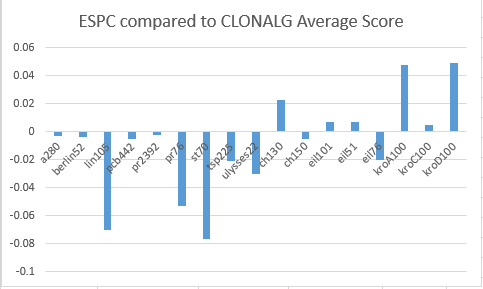
\includegraphics[]{Images/ESPC_Fig_Avg.png}
\label{ESCP_AVG}
\caption{MAE on Average Score for ESPC compared to CLONALG}
\end{figure}
\begin{figure}[H]
	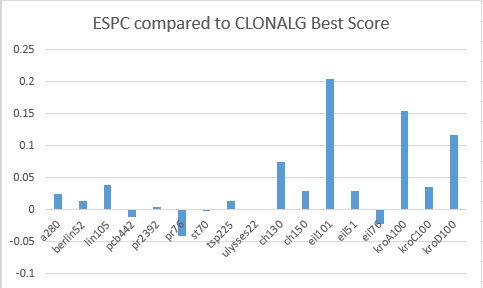
\includegraphics[]{Images/ESPC_Fig_Best.png}
	\label{ESCP_Best}
	\caption{MAE on Best Score for ESPC compared to CLONALG}
\end{figure}
\begin{figure}[H]
	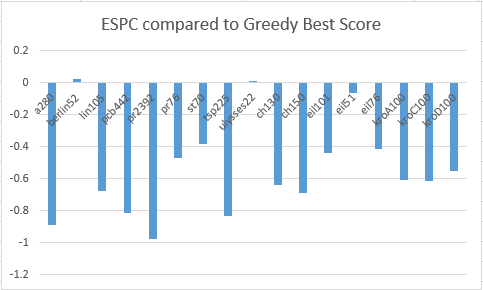
\includegraphics[]{Images/ESPC_Fig_Greedy.png}
	\label{ESCP_Greedy}
	\caption{MAE on Best Score for ESPC compared to Greedy}
\end{figure}
\begin{table}[H]
	\begin{tabular}{|l|p{2cm}|p{1.6cm}|p{2.2cm}|p{2.4cm}|p{2.4cm}|p{1.7cm}|}
		\hline
		TSP       & Average Score & Best Score & Best Percentage & MAE compared to CLONALG & MAE on Best Score & Average Evalutions \\ \hline
		a280      & 26559.75      & 24949      & 867.3904614     & -0.002852436            & 0.025331677       & 34025.59           \\ \hline
		berlin52  & 11120.65      & 9241       & 22.52718112     & -0.003905347            & 0.013851315       & 173022.70          \\ \hline
		lin105    & 74683.73      & 60638      & 321.7122192     & -0.070331918            & 0.038639137       & 48963.38           \\ \hline
		pcb442    & 652981.26     & 637838     & 1156.130608     & -0.005310796            & -0.010447794      & 35590.02           \\ \hline
		pr2392    & 14259316.88   & 14060841   & 3619.484329     & -0.001940763            & 0.004410689       & 31152.73           \\ \hline
		pr76      & 316531.58     & 278997     & 157.9507947     & -0.052809423            & -0.040201149      & 64605.41           \\ \hline
		st70      & 1912.1        & 1511       & 123.8518519     & -0.076884054            & -0.000661813      & 68687.03           \\ \hline
		tsp225    & 31963.99      & 29509      & 653.5495403     & -0.020461463            & 0.013419635       & 36970.86           \\ \hline
		ulysses22 & 7499.74       & 6901       & 0               & -0.030227715            & 0                 & 27280.05           \\ \hline
		ch130     & 30748.35      & 27332      & 347.3322422     & 0.022916677             & 0.075332943       & 45024.26           \\ \hline
		ch150     & 38069.35      & 34981      & 435.8609069     & -0.00488871             & 0.029558903       & 40273.29           \\ \hline
		eil101    & 2111.16       & 1622       & 157.8696343     & 0.007285094             & 0.204685573       & 53395.42           \\ \hline
		eil51     & 650.27        & 536        & 25.82159624     & 0.006735664             & 0.029850746       & 118097.23          \\ \hline
		eil76     & 1405.74       & 1221       & 126.9516729     & -0.020167314            & -0.022113022      & 62993.43           \\ \hline
		kroA100   & 91818.4       & 75100      & 252.8803684     & 0.047880163             & 0.15412783        & 62252.60           \\ \hline
		kroC100   & 94006.78      & 82471      & 297.4697576     & 0.004941665             & 0.035127499       & 57812.68           \\ \hline
		kroD100   & 88897.32      & 75500      & 254.5599699     & 0.049322972             & 0.116622517       & 58883.91           \\ \hline
	\end{tabular}
	\caption{ESPC performance}
	\label{tab:espc}
\end{table}
